
\providecommand{\Fun}{\operatorname{Fun}}
\providecommand{\Cat}{\mathcal{C}at}
\providecommand{\sSet}{s\mathcal{S}et}
\providecommand{\Set}{\mathcal{S}et}
\providecommand{\QCat}{\mathcal{Q}\mathcal{C}at}
\providecommand{\ssSet}{ss\mathcal{S}et}%
\providecommand{\CSS}{\mathcal{C}\mathcal{S}\mathcal{S}}
\providecommand{\OneComp}{1\text{-}\mathcal{C}omp}
\providecommand{\qcOne}{\mathbf{1}}   %
\providecommand{\qcInt}{\mathbb{I}}   %
\providecommand{\rvWarrow}{\rightsquigarrow}%

\section{\texorpdfstring{$(\infty,n)$}{(∞,n)}-\trCategory{}的%
\trInfinityCosmos}\label{sec:infinity-cosmoi-of-infinity-n-categories}

在本节中，我们引入各式各样的\trInfinityCosmos，其对象是一些 $(\infty,n)$-%
\trCategory（$1<n\le\oo$）的模型。这些\trInfinityCosmos{}描述了诸%
\trInfinityCategory、诸\trInfinityFunctor{}与诸\trInfinityNaturalTransformation{}%
的 $(\infty,2)$-\trCategory，其间略去更高维的变换；不过，诸\trGeneralizedElement{}%
与诸\trInternalHom{}仍使我们得以触及高维的非可逆态射。

由于完整地规定一个 $(\infty,n)$-\trCategory{}的模型所牵涉的组合学可能相当繁难，
为省篇幅，我们不对这里讨论的每一个高阶范畴论概念都给出定义，而是提供指出这些
定义所在之处的外部引注。

我们的几个 $(\infty,n)$-\trCategory{}模型被定义为经一个 1-\trCategory{}
$\boldsymbol{\Theta}_{n}$ 所索引的预层——该\trCategory{}由 Joyal 在一篇未发表的
札记中最先引入 \cite{bib60}，我们这里呈献的是归于 Berger 的一个等价形式
\cite{bib11}。

\begin{definition}\label{def:theta-categories}
对 $0\le n\le\oo$，归纳地定义一族 1-\trCategory{} $\boldsymbol{\Theta}_{n}$ 如下。
\begin{itemize}
\item $\boldsymbol{\Theta}_{0}\coloneqq\qcOne$ 是\trTerminal{}范畴，而
  $\boldsymbol{\Theta}_{1}\coloneqq\Delta$ 是由有限非空序数与保序映射构成的%
  \trCategory。
\item $\boldsymbol{\Theta}_{n}\coloneqq\Delta\wr\boldsymbol{\Theta}_{n-1}$，其中
  $\Delta\wr\text{--}\colon\Cat\to\Cat$ 是\textbf{\trWreathProduct}（categorial
  wreath product）构造。显式地，对一个 1-\trCategory{} $C$，$\Delta\wr C$
  是这样的\trCategory：
  \begin{itemize}
  \item 其对象是诸二元组 $[n](c_{1},\dots,c_{n})$，其中 $[n]\in\Delta$ 且
    $c_{i}\in C$；
  \item 其态射 $(\alpha;\bar{f})\colon[n](c_{1},\dots,c_{n})\to[m](c'_{1},\dots,c'_{m})$ 由一个单纯映射
    $\alpha\colon[n]\to[m]\in\Delta$
    连同诸态射 $f_{i,j}\colon c_{i}\to c'_{j}\in C$ 给出，后者对一切
    $0<i\le n$ 与 $\alpha(i-1)<j\le\alpha(i)$。
  \end{itemize}
\end{itemize}
\end{definition}

$\boldsymbol{\Theta}_{n}$ 的对象定义 $0\le k\le n$ 时 k-\trCell{}的%
\trPastingDiagram，而其态射定义投影、复合与退化映射。把一个\trPastingDiagram{}%
送到由它生成的自由严格 $n$-\trCategory{}的那个\trFunctor{}
$\boldsymbol{\Theta}_{n}\to n\text{-}\Cat$ 是\trFullyFaithful{}
\cite[3.7]{bib11}。

例如，$\boldsymbol{\Theta}_{2}$ 中的态射
$(\delta^{2};(\delta^{1},!,\mathrm{id}))\colon[2]([1],[1])\to[3]([2],[0],[1])$
对应于由下列\trPastingDiagram{}所生成的自由 2-\trCategory{}之间的一个%
\trTwoFunctor：
\begin{center}
\begin{tikzpicture}[x=1.9em,y=1.3em]
  \node (a0) at (0,0) {$0$};
  \node (a1) at (2.6,0) {$1$};
  \node (a2) at (5.2,0) {$2$};
  \draw[->] (0.45,0.18) -- (2.15,0.18);
  \draw[->] (0.45,-0.18) -- (2.15,-0.18);
  \node at (1.3,0) {$\scriptstyle\Downarrow$};
  \draw[->] (3.05,0.18) -- (4.75,0.18);
  \draw[->] (3.05,-0.18) -- (4.75,-0.18);
  \node at (3.9,0) {$\scriptstyle\Downarrow$};
  \node at (7.1,0) {$\mapsto$};
  \begin{scope}[shift={(8.8,0)}]
    \node (b0) at (0,0) {$0$};
    \node (b1) at (2.6,0) {$1$};
    \node (b2) at (5.2,0) {$2$};
    \node (b3) at (7.8,0) {$3$};
    \draw[->] (0.45,0.18) -- (2.15,0.18);
    \draw[->] (0.45,-0.18) -- (2.15,-0.18);
    \node at (1.3,0.55) {$\scriptstyle\Downarrow$};
    \node at (1.3,-0.55) {$\scriptstyle\Downarrow$};
    \draw[->] (3.05,0) -- (4.75,0);
    \draw[->] (5.65,0.18) -- (7.35,0.18);
    \draw[->] (5.65,-0.18) -- (7.35,-0.18);
    \node at (6.5,0) {$\scriptstyle\Downarrow$};
  \end{scope}
\end{tikzpicture}
\end{center}
它把 0 送到 0、把 1 送到 1、把 2 送到 3，并把定义域的左 2-\trCell{}送到余定义域
最左侧诸 2-\trCell{}的竖直复合，把定义域的右 2-\trCell{}送到余定义域最右侧的
2-\trCell{}与中央 1-\trCell{}的\trWhiskering。

\begin{lemma}\label{lem:wreath-product-adjunction}
对任何带有一个\trTerminal{}元素 $t$ 的 1-\trCategory，下方左侧的\trAdjunction{}%
诱导下方右侧的\trAdjunction：
\begin{center}
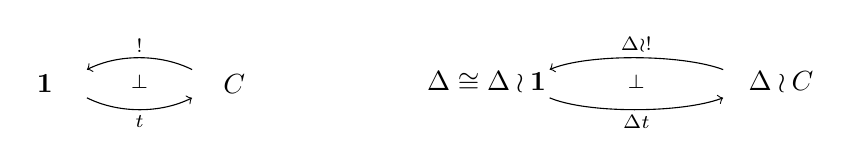
\begin{tikzpicture}[x=1.9em,y=1.5em]
  \node (a) at (0,0) {$\qcOne$};
  \node (b) at (3.6,0) {$C$};
  \draw[->] (2.8,0.34) .. controls (2.2,0.72) and (1.4,0.72) .. (0.8,0.34);
  \node at (1.8,0.92) {$\scriptstyle!$};
  \node at (1.8,0.05) {$\scriptstyle\bot$};
  \draw[->] (0.8,-0.34) .. controls (1.4,-0.72) and (2.2,-0.72) .. (2.8,-0.34);
  \node at (1.8,-0.92) {$\scriptstyle t$};
  \node at (5.7,0) {$\rvWarrow$};
  \begin{scope}[shift={(8.4,0)}]
    \node (c) at (0,0) {$\Delta\cong\Delta\wr\qcOne$};
    \node (d) at (5.6,0) {$\Delta\wr C$};
    \draw[->] (4.5,0.34) .. controls (3.7,0.72) and (1.9,0.72) .. (1.2,0.34);
    \node at (2.85,0.92) {$\scriptstyle\Delta\wr!$};
    \node at (2.85,0.05) {$\scriptstyle\bot$};
    \draw[->] (1.2,-0.34) .. controls (1.9,-0.72) and (3.7,-0.72) .. (4.5,-0.34);
    \node at (2.85,-0.92) {$\scriptstyle\Delta t$};
  \end{scope}
\end{tikzpicture}
\end{center}
\end{lemma}
\begin{proof}
\trWreathProduct{}定义一个 2-\trFunctor{}
$\Delta\wr\text{--}\colon\Cat\to\Cat$。
\end{proof}

Ara 引入了一个对每个 $1\le n<\oo$ 的 $(\infty,n)$-\trCategory{}之模型，称作
\textbf{$n$-拟范畴}（$n$-quasi-categories），即 $\boldsymbol{\Theta}_{n}$ 之上由
一个特别的右\trLifting{}性质所刻画的预层，该性质描述于 \cite[\S5]{bib4}。
Ara 的 1-拟范畴与通常的\trQuasiCategory{}相重合。

\begin{proposition}\label{prop:n-quasi-category-cosmos}
对每个 $n\ge 1$，诸 $n$-拟范畴的全子范畴
$n\text{-}\QCat\hookrightarrow\Set^{\boldsymbol{\Theta}_{n}^{\mathrm{op}}}$
定义一个\trCartesianClosed{}\trInfinityCosmos。
\end{proposition}
\begin{proof}
Ara 在\trCategory{}
$\Set^{\boldsymbol{\Theta}_{n}^{\mathrm{op}}}$ 上构造了一个\trCartesianClosed{}%
\trModelStructure——它在 $n=1$ 的情形推广了 Joyal \trModelStructure——其中诸%
\trFibrant{}对象恰是诸 $n$-拟范畴，而诸余纤维化是诸\trMonomorphism{}
\cite{bib4}；特别地，一切对象皆\trCofibrant。于是，要在全子范畴
$n\text{-}\QCat$ 上诱导一个\trCartesianClosed{}\trInfinityCosmos{}结构，
只须找到一支从这一\trModelStructure{}通往拟范畴之\trModelStructure{}的
Quillen \trAdjunction，使其\trLeftAdjoint{}
$\Set^{\Delta^{\mathrm{op}}}\to\Set^{\boldsymbol{\Theta}_{n}^{\mathrm{op}}}$ 保持
二元\trProduct。

为此，注意到 $[0]\in\boldsymbol{\Theta}_{n-1}$ 对一切 $n>1$ 是\trTerminal{}的，
于是\cref{lem:wreath-product-adjunction}提供了如下方左侧的一个\trAdjunction，
从而也提供了如下方右侧的一个\trAdjunction：
\begin{center}
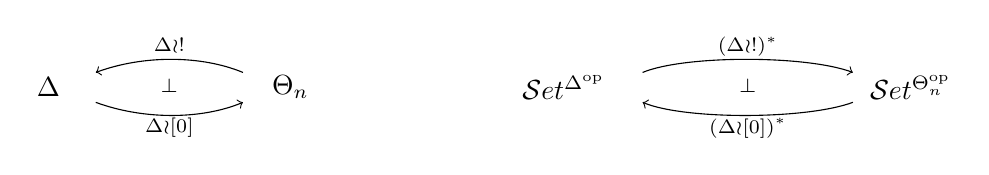
\begin{tikzpicture}[x=1.9em,y=1.5em]
  \node (d) at (0,0) {$\Delta$};
  \node (t) at (4.6,0) {$\boldsymbol{\Theta}_{n}$};
  \draw[->] (3.7,0.36) .. controls (2.9,0.78) and (1.8,0.78) .. (0.9,0.36);
  \node at (2.3,0.98) {$\scriptstyle\Delta\wr!$};
  \node at (2.3,0.05) {$\scriptstyle\bot$};
  \draw[->] (0.9,-0.36) .. controls (1.8,-0.78) and (2.9,-0.78) .. (3.7,-0.36);
  \node at (2.3,-0.98) {$\scriptstyle\Delta\wr[0]$};
  \node at (7.0,0) {$\rvWarrow$};
  \begin{scope}[shift={(9.8,0)}]
    \node (s) at (0,0) {$\Set^{\Delta^{\mathrm{op}}}$};
    \node (p) at (6.6,0) {$\Set^{\boldsymbol{\Theta}_{n}^{\mathrm{op}}}$};
    \draw[->] (1.5,0.36) .. controls (2.3,0.78) and (4.6,0.78) .. (5.5,0.36);
    \node at (3.5,0.98) {$\scriptstyle(\Delta\wr!)^{\ast}$};
    \node at (3.5,0.05) {$\scriptstyle\bot$};
    \draw[->] (5.5,-0.36) .. controls (4.6,-0.78) and (2.3,-0.78) .. (1.5,-0.36);
    \node at (3.5,-0.98) {$\scriptstyle(\Delta\wr[0])^{\ast}$};
  \end{scope}
\end{tikzpicture}
\end{center}
\trRightAdjoint{}
$\Delta\wr[0]\colon\Delta\hookrightarrow\boldsymbol{\Theta}_{n}$ 把 $\Delta$ 包含
为「仅由 1-\trCell{}组成的\trPastingDiagram」之子范畴；于是，沿这一\trFunctor{}%
的限制 $(\Delta\wr[0])^{\ast}\colon\Set^{\boldsymbol{\Theta}_{n}^{\mathrm{op}}}\to\Set^{\Delta^{\mathrm{op}}}$ 忘掉高维胞腔。另一支伴随
$\Delta\wr!\colon\boldsymbol{\Theta}_{n}\to\Delta$ 投影到\trWreathProduct{}的第一分量上。
注意到预层\trCategory{}之间相应的限制\trFunctor{}拥有它自己的一个\trLeftAdjoint%
——由左\trKanExtension{}所定义——从而显然保持诸\trProduct。

的确，出于同一理由，这一\trLeftAdjoint{}保持一切\trLimit，从而也保持诸%
\trMonomorphism（它们可以刻画为其\trKernelPair（kernel pair）由恒同给出的那些映射）。
据 Joyal 与 Tierney 的一个结果 \cite[7.15]{bib64}，要证明一支\trAdjunction{}是
Quillen 的，只须证明其\trLeftAdjoint{}保持诸余纤维化——如我们刚刚所做的——
而其\trRightAdjoint{}保持\trFibrant{}对象之间的诸\trFibration。据
\cref{lem:adjunction-transposes-lifting}，这意味着我们只须验证：这一%
\trLeftAdjoint{}把诸内号角包含
$\{\Lambda^{k}[n]\hookrightarrow\Delta[n]\}_{n\ge2,0<k<n}$ 与映射
$\qcOne\hookrightarrow\qcInt$ 载为 Ara 的\trModelStructure{}中的诸平凡余纤维化。
事实上，由 \cite[3.5]{bib64}，只须考虑诸脊柱包含
$\{\Gamma[n]\hookrightarrow\Delta[n]\}_{n\ge2}$ 以替代诸内号角包含——我们也将
如此行事。

为看到这一点，有益的是注意到——如 \cite[\S6]{bib4} 中所观察——这一%
\trLeftAdjoint{}与严格 1-\trCategory{}和严格 $n$-\trCategory{}的诸神经嵌入相
交换：
\begin{center}
\begin{tikzpicture}[x=1.9em,y=1.5em]
  \node (cat)  at (0,1.4) {$\Cat$};
  \node (ncat) at (5.8,1.4) {$n\text{-}\Cat$};
  \node (setd) at (0,-1.4) {$\Set^{\Delta^{\mathrm{op}}}$};
  \node (sett) at (5.8,-1.4) {$\Set^{\boldsymbol{\Theta}_{n}^{\mathrm{op}}}$};
  \draw[right hook->] (0.95,1.4) -- (4.75,1.4);
  \draw[->] (ncat) -- (sett);
  \draw[right hook->] (cat) -- (setd);
  \draw[->] (1.7,-1.4) -- node[above]{$\scriptstyle(\Delta\wr[0])^{\ast}$} (4.0,-1.4);
\end{tikzpicture}
\end{center}
特别地，这一\trLeftAdjoint{}把 $\qcOne\hookrightarrow\qcInt$ 的 1-范畴性神经
送到这一映射的严格 $n$-范畴性神经；而且，由于这一\trLeftAdjoint{}也保持诸%
\trColimit，它把脊柱包含 $\Gamma[n]\hookrightarrow\Delta[n]$ 送到对象
$[n]([0],\dots,[0])\in\boldsymbol{\Theta}_{n}$ 的相应的「脊柱包含」。由于这两类
映射都属于 Ara 的「$n$-拟范畴的\trLocalizer」（\cite[5.17]{bib4}），它们必定是
平凡余纤维化。于是，这支伴随如所断言是 Quillen 的，而\cref{cor:cartesian-closed-cosmos}%
适用于在 $n\text{-}\QCat$ 上创造一个\trCartesianClosed{}\trInfinityCosmos{}%
结构。
\end{proof}

另一类 $(\infty,n)$-\trCategory{}的模型，对 $0\le n<\oo$，归于 Rezk
\cite{bib101}。一个\textbf{$\boldsymbol{\Theta}_{n}$-空间}（$\boldsymbol{\Theta}_{n}$-space）
是 $\boldsymbol{\Theta}_{n}$ 上的一个单纯预层，满足与\cref{def:complete-segal-space}%
的那些条件相类比的 Reedy 纤维性、Segal 与完全性诸条件。一个
$\boldsymbol{\Theta}_{1}$-空间恰是一个\trCompleteSegalSpaces，而一个
$\boldsymbol{\Theta}_{0}$-空间只不过是一个\trKanComplex。

\begin{proposition}\label{prop:theta-space-cosmos}
对每个 $n\ge 1$，诸 $\boldsymbol{\Theta}_{n}$-空间的全子范畴
$\boldsymbol{\Theta}_{n}\text{-}\mathcal{S}p\hookrightarrow\ssSet^{\boldsymbol{\Theta}_{n}^{\mathrm{op}}}$ 定义一个\trCartesianClosed{}%
\trInfinityCosmos，对其而言，底\trCompleteSegalSpaces{}函子
$U\colon\boldsymbol{\Theta}_{n}\text{-}\mathcal{S}p\to\boldsymbol{\Theta}_{1}\text{-}\mathcal{S}p\cong\CSS$ 是\trCosmological。
\end{proposition}
\begin{proof}
Rezk 在\trCategory{}
$\ssSet^{\boldsymbol{\Theta}_{n}^{\mathrm{op}}}$ 上构造了一个\trCartesianClosed{}%
\trModelStructure，它在 $n=1$ 的情形推广了他的\trCompleteSegalSpaces{}之%
\trModelStructure，其中诸\trFibrant{}对象恰是诸 $\boldsymbol{\Theta}_{n}$-空间，
而诸余纤维化是诸\trMonomorphism{} \cite{bib101}；特别地，一切对象皆%
\trCofibrant。于是，要在全子范畴 $\boldsymbol{\Theta}_{n}\text{-}\mathcal{S}p$ 上
诱导一个\trCartesianClosed{}\trInfinityCosmos{}结构，只须找到一支介于这一%
\trModelStructure{}与\trCompleteSegalSpaces{}之\trModelStructure{}之间的
Quillen \trAdjunction，使其\trLeftAdjoint{}
$\sSet^{\Delta^{\mathrm{op}}}\to\ssSet^{\boldsymbol{\Theta}_{n}^{\mathrm{op}}}$
保持二元\trProduct。随后，我们把这一伴随与伴随 \eqref{eq:pi-iota-adjunction}
的复合施用\cref{cor:cartesian-closed-cosmos}。

一如\cref{prop:n-quasi-category-cosmos}的证明，我们经由把
\cref{lem:wreath-product-adjunction}施用于\trTerminal{}对象
$[0]\in\boldsymbol{\Theta}_{n-1}$ 而得到所需的伴随：
\begin{rveq}\label{eq:theta-space-adjunction}
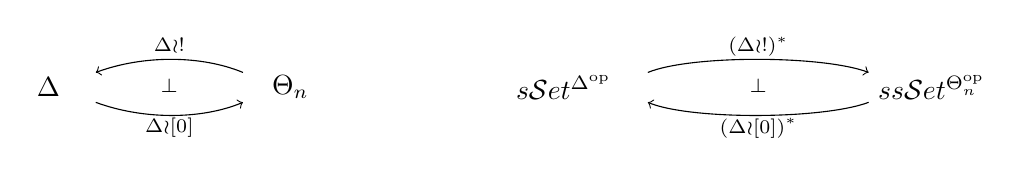
\begin{tikzpicture}[x=1.9em,y=1.5em]
  \node (d) at (0,0) {$\Delta$};
  \node (t) at (4.6,0) {$\boldsymbol{\Theta}_{n}$};
  \draw[->] (3.7,0.36) .. controls (2.9,0.78) and (1.8,0.78) .. (0.9,0.36);
  \node at (2.3,0.98) {$\scriptstyle\Delta\wr!$};
  \node at (2.3,0.05) {$\scriptstyle\bot$};
  \draw[->] (0.9,-0.36) .. controls (1.8,-0.78) and (2.9,-0.78) .. (3.7,-0.36);
  \node at (2.3,-0.98) {$\scriptstyle\Delta\wr[0]$};
  \node at (7.0,0) {$\rvWarrow$};
  \begin{scope}[shift={(9.8,0)}]
    \node (s) at (0,0) {$\sSet^{\Delta^{\mathrm{op}}}$};
    \node (p) at (7.0,0) {$\ssSet^{\boldsymbol{\Theta}_{n}^{\mathrm{op}}}$};
    \draw[->] (1.6,0.36) .. controls (2.4,0.78) and (4.9,0.78) .. (5.8,0.36);
    \node at (3.7,0.98) {$\scriptstyle(\Delta\wr!)^{\ast}$};
    \node at (3.7,0.05) {$\scriptstyle\bot$};
    \draw[->] (5.8,-0.36) .. controls (4.9,-0.78) and (2.4,-0.78) .. (1.6,-0.36);
    \node at (3.7,-0.98) {$\scriptstyle(\Delta\wr[0])^{\ast}$};
  \end{scope}
\end{tikzpicture}
\end{rveq}
其\trLeftAdjoint{}拥有一个更进一层的\trLeftAdjoint——由左\trKanExtension{}所
给出——从而保持诸\trProduct。

尚须论证的只是这支伴随是 Quillen 的。$\boldsymbol{\Theta}_{n}$-空间之%
\trModelStructure——并且，经特化，\trCompleteSegalSpaces{}之%
\trModelStructure——被定义为单纯预层上内射（或者等价地，Reedy）%
\trModelStructure{}的一个\trBousfieldLocalization。在\trInjectiveModelStructure{}中，
诸余纤维化与诸平凡余纤维化在 $\sSet$ 中逐点定义，故这一\trLeftAdjoint{}相对
于这些\trModelStructure{}显然是左 Quillen 的。于是，这支伴随对局部化后的诸%
\trModelStructure{}是 Quillen 的，当且仅当其\trRightAdjoint{}——即 Rezk 称作
「底单纯空间」的那个\trFunctor——保持诸\trFibrant{}对象；因为在此情形，这一%
\trLeftAdjoint{}保持新的诸平凡余纤维化，而后者正是由前者来定义的。一个函子
$X\in\ssSet^{\boldsymbol{\Theta}_{n}^{\mathrm{op}}}$ 是\trFibrant{}的，当且仅当它
满足 Reedy、Segal 与完全性诸条件。由于伴随 \eqref{eq:theta-space-adjunction}
对内射/Reedy \trModelStructure{}是 Quillen 的，Reedy 纤维性条件得以保持，而
Rezk 证明了 Segal 条件也得以保持 \cite[7.2]{bib101}。诸 $\boldsymbol{\Theta}_{n}$%
-空间的完全性条件由底单纯空间的完全性条件所创造 \cite[\S7]{bib101}，故这一
条件同样得以保持。于是，\trRightAdjoint{} \eqref{eq:theta-space-adjunction}
限制为一个函子 $U\colon\boldsymbol{\Theta}_{n}\text{-}\mathcal{S}p\to\CSS$，我们
称之为\textbf{底\trCompleteSegalSpaces{}函子}（underlying complete Segal
space functor）。

\cref{cor:cartesian-closed-cosmos}适用于在
$\boldsymbol{\Theta}_{n}\text{-}\mathcal{S}p$ 上创造一个\trCartesianClosed{}%
\trInfinityCosmos{}结构。由\cref{lem:finite-product-adjunction-v-enriched}，
伴随 \eqref{eq:theta-space-adjunction} 富集于双单纯集之上，于是
\cref{prop:change-of-base-model-cosmoi}可用来证明底\trCompleteSegalSpaces{}%
函子是\trCosmological。
\end{proof}

还存在另一个 $(\infty,n)$-\trCategory{}的模型，它推广了 $(\infty,1)$-%
\trCategory{}的\trCompleteSegalSpaces{}模型，并利用了取值于一个\trModelCategory{}%
中的\textbf{\trRezkObject}（Rezk object）这一概念：

\begin{definition}\label{def:rezk-objects}
设 $\mathcal{M}$ 是一个\trModelCategory。
\begin{enumerate}[label=(\roman*)]
\item 一个\trSimplicialObject{}
  $X_{\bullet}\in\mathcal{M}^{\Delta^{\mathrm{op}}}$ 是\textbf{Reedy 纤维性}的，
  恰当其在诸\trWeightedLimit{}上诱导的映射
  \[
  X_{m}\cong\operatorname{lim}_{\Delta[m]}X\longrightarrow
  \operatorname{lim}_{\partial\Delta[m]}X=:\ M_{m}X
  \]
  对一切 $m\ge 0$ 都是一个\trFibration。
\item 一个 Reedy 纤维性的\trSimplicialObject{} $X_{\bullet}$ 是一个%
  \textbf{\trSegalObject}（Segal object），恰当其在诸\trWeightedLimit{}上诱导的
  映射
  \[
  X_{n}\cong\operatorname{lim}_{\Delta[n]}X\longrightarrow
  \operatorname{lim}_{\Lambda^{k}[n]}X
  \]
  对一切 $n\ge 2$ 与 $0<k<n$ 都是一个\trTrivialFibration。
\item 一个\trSegalObject{} $X_{\bullet}$ 是一个\textbf{\trRezkObject}，恰当其在诸%
  \trWeightedLimit{}上诱导的映射
  \[
  \operatorname{lim}_{\qcInt}X\longrightarrow
  \operatorname{lim}_{\Delta[0]}X\cong X_{0}
  \]
  是一个\trTrivialFibration。
\end{enumerate}
\end{definition}

一个映射 $p\colon X_{\bullet}\to Y_{\bullet}\in\mathcal{M}^{\Delta^{\mathrm{op}}}$
是一个\textbf{\trRezkIsofibration}（Rezk isofibration），若出现于 (i)、(ii) 与
(iii) 中的那些映射的相对类比——它们由 $p$ 与相应的诸权之映射所作的 Leibniz
加权\trWeightedLimit{}而形成——分别是\trFibration、\trTrivialFibration{}与一个%
\trTrivialFibration。

我们对\cref{def:complete-segal-space}的表述与 Rezk 对其诸条件的原有框架略有
出入，其意在使人看清：诸\trCompleteSegalSpaces{}恰好是取值于 Quillen 的%
\trKanComplex{}之\trModelStructure{}中的诸\trRezkObject。

\begin{proposition}\label{prop:rezk-cosmos}
试设 $\mathcal{M}$ 是一个 \emph{\trCisinskiModelCategory}。\footnote{一个%
\textbf{\trCisinskiModelStructure}（Cisinski model structure）是一个%
\trGrothendieckTopos（Grothendieck topos）上的组合模型结构，其中诸余纤维化恰是诸%
\trMonomorphism。由此可得：$\mathcal{M}^{\Delta^{\mathrm{op}}}$ 上的 Reedy
\trModelStructure{}与\trInjectiveModelStructure{}相重合，并且特别地，一切对象皆%
\trCofibrant{} \cite{bib27,bib16}。}于是，诸\trRezkObject{}的全子范畴
$\mathcal{R}ezk_{\mathcal{M}}\hookrightarrow\mathcal{M}^{\Delta^{\mathrm{op}}}$
定义一个\trInfinityCosmos。
\end{proposition}
\begin{proof}
我们直接从\cref{prop:fibrant-objects-cosmos}出发证明这一结果，办法是证明：
$\mathcal{M}^{\Delta^{\mathrm{op}}}$ 上 Reedy \trModelStructure{}的一个%
\trBousfieldLocalization{}定义一个\trCisinskiModelStructure，它富集于拟范畴之%
\trModelStructure{}之上，而其\trFibrant{}对象恰是诸\trRezkObject。

首先，观察到\trCategory{}
$\mathcal{M}^{\Delta^{\mathrm{op}}}$ 是单纯富集、单纯张量且单纯余张量的，其
hom-空间被富于暗示地记作「$\Fun$」：
\[
(\otimes,\{,\},\Fun)\colon\sSet\times\mathcal{M}^{\Delta^{\mathrm{op}}}
\to\mathcal{M}^{\Delta^{\mathrm{op}}}
\]
并且使得单纯集的诸\trMonomorphism{}与（平凡的）Reedy 余纤维化的 Leibniz
张量是（平凡的）Reedy 余纤维化 \cite[4.4]{bib35}。我们施用 Jeff Smith 定理
\cite{bib8} 证明 $\mathcal{M}^{\Delta^{\mathrm{op}}}$ 容有一个模型结构，其中：
\begin{itemize}
\item 诸余纤维化是诸\trMonomorphism；
\item 诸\trFibrant{}对象是诸\trRezkObject；
\item \trFibrant{}对象之间的诸\trFibration{}是诸\trRezkIsofibration；并且
\item 诸\trWeakEquivalence{}是诸 \textbf{\trRezkWeakEquivalence}（Rezk weak
  equivalences），即那些对一切\trRezkObject{} $X$ 都诱导\trQuasiCategory{}的一个%
  \trEquivalence{} $w^{\ast}\colon\Fun(V,X)\to\Fun(U,X)$ 的映射
  $w\colon U\to V$。
\end{itemize}

注意到，由伴随，一个映射 $p\colon X\to Y\in\mathcal{M}^{\Delta^{\mathrm{op}}}$
是一个\trRezkIsofibration，当且仅当对 $\mathcal{M}$ 中的一切\trMonomorphism{}
$m\colon A\to B$，单纯集之诱导映射
\[
\Fun(B,X)\xrightarrow{\ \widehat{\Fun}(m,p)\ }
\Fun(A,X)\times_{\Fun(A,Y)}\Fun(B,Y)
\]
是\trQuasiCategory{}之间的一个\trIsofibration。据\cref{cor:leibniz-anodyne}与%
\cref{prop:leibniz-stability-isofibrations}，这成立当且仅当该映射对集合
$I\mathbin{\widehat{\times}}J$ 中的映射具有右\trLifting{}性质，其中
\[
I\coloneqq\{\partial\Delta[n]\hookrightarrow\Delta[n]\}_{n\ge0}
\qquad\text{以及}\qquad
J\coloneqq\{\Lambda^{k}[n]\hookrightarrow\Delta[n]\}_{n\ge2,0<k<n}
\cup\{\qcOne\hookrightarrow\qcInt\}.
\]

再次由伴随，以及\cref{prop:leibniz-construction-preserves}(i)，$p$ 是一个%
\trRezkIsofibration，当且仅当它对诸映射之集
$(i\mathbin{\widehat{\times}}j)_{\ast}m\cong j\mathbin{\widehat{\times}}(i_{\ast}m)$——其中 $i\in I$、$j\in J$，而 $m$
取遍 $\mathcal{M}$ 中的生成余纤维化——具有右\trLifting{}性质，这里 $\ast$
表示点态张量 $\ast\colon\sSet\times\mathcal{M}\to\mathcal{M}^{\Delta^{\mathrm{op}}}$。由于据\cref{prop:reedy-cellularly-generated}，
$\mathcal{M}^{\Delta^{\mathrm{op}}}$ 中的诸 Reedy 余纤维化由诸映射 $i_{\ast}m$
（$i\in I$，而 $m$ 取遍 $\mathcal{M}$ 中的生成余纤维化）之集所胞腔式生成，我们
由伴随得出结论：$p$ 是\trRezkObject{}之间的一个\trRezkIsofibration，当且仅当
\[
\Fun(V,X)\xrightarrow{\ \widehat{\Fun}(c,p)\ }
\Fun(U,X)\times_{\Fun(U,Y)}\Fun(V,Y)
\]
对 $\mathcal{M}^{\Delta^{\mathrm{op}}}$ 中的一切\trMonomorphism{}
$c\colon U\to V$ 都是\trIsofibration。

现在容易验证 Jeff Smith 定理的诸条件。诸\trRezkWeakEquivalence{}是\trAccessible{}且满足%
\trTwoOfThreeProperty。我们论证：诸\trRezkWeakEquivalence{}包含一切 Reedy 弱等价，从而
包含诸 Reedy 平凡纤维化——后者由对诸\trMonomorphism{}的右\trLifting{}性质所
刻画。转置 \cite[4.4]{bib35} 中已就 $\mathcal{M}^{\Delta^{\mathrm{op}}}$ 上的
Reedy \trModelStructure{}所作的诸观察，我们看到：对任何 Reedy 平凡余纤维化
$w\colon U\to V$ 与\trRezkObject{} $X$，$w^{\ast}\colon\Fun(V,X)\to\Fun(U,X)$ 是%
\trQuasiCategory{}之间的一个\trEquivalence。据 Ken Brown \cref{lem:ken-brown}，
当 $w$ 只是一个 Reedy 弱等价时亦然。注意到，一个映射 $w\colon U\to V$ 既是%
\trRezkWeakEquivalence{}又是余纤维化，恰当 $w^{\ast}\colon\Fun(V,X)\to\Fun(U,X)$ 是%
\trQuasiCategory{}之间的一个\trTrivialFibration。这一刻画证明了：诸%
\trRezkWeakEquivalence{}与诸余纤维化组成的类对推出与超限复合封闭。Jeff Smith 定理由此蕴含：
诸\trRezkObject{}的模型结构存在。

要看到\trRezkObject{}的模型结构富集于拟范畴之\trModelStructure{}之上，我们必须
验证
\[
(\otimes,\{,\},\Fun)\colon\sSet\times\mathcal{M}^{\Delta^{\mathrm{op}}}
\to\mathcal{M}^{\Delta^{\mathrm{op}}}
\]
定义一个 Quillen 双变量\trAdjunction（见\cref{def:quillen-two-variable-adjunction}）。
局部化后的\trRezkObject{}之\trModelStructure{}中的诸余纤维化与 $\mathcal{M}^{\Delta^{\mathrm{op}}}$
上 Reedy \trModelStructure{}的诸余纤维化相同，故我们已然知道：诸余纤维化的
Leibniz 张量是余纤维化。为验证这一公理的其余 2/3，我们援引 Dugger 的一个结果
\cite[3.2]{bib35}，它告诉我们：在头一个 1/3 在场的情形下，要验证单纯集的诸%
\trMonomorphism{}与诸平凡余纤维化之 Leibniz 张量是平凡余纤维化，只须证明单纯
余张量 $(\text{--})^{K}\colon\mathcal{M}^{\Delta^{\mathrm{op}}}\to\mathcal{M}^{\Delta^{\mathrm{op}}}$
保持纤维性对象之间的诸\trFibration。对于\trBousfieldLocalization，\trRezkObject{}之间的%
\trRezkIsofibration{}与\trRezkObject{}之间的 Reedy \trFibration{}相重合%
\cite[3.3.16]{bib55}。经直接验证易知 $(\text{--})^{K}$ 保持\trRezkObject，而
Reedy 纤维化之保持则是我们已知的事实之一。

对于 Quillen 双变量\trAdjunction{}的最后 1/3，我们使用 Dugger 结果的第二部分
\cite[3.2]{bib35}，它告诉我们：在前 2/3 在场的情形下，只须验证：对一切%
\trRezkObject{} $Z$ 与单纯集的平凡余纤维化 $j\colon J\to K$，映射
$Z^{j}\colon Z^{K}\to Z^{J}$ 是一个\trRezkWeakEquivalence（这里须假设
$\mathcal{M}^{\Delta^{\mathrm{op}}}$ 是左固有的，而此处情形正是如此，因为一切
对象皆\trCofibrant）。事实上，我们可以证明这一映射是一个\trTrivialFibration：
检验它对诸\trMonomorphism{} $c\colon U\to V\in\mathcal{M}^{\Delta^{\mathrm{op}}}$
的右\trLifting{}性质即可。经转置我们看到：$c$ 对 $Z^{j}$ 可提升，当且仅当 $j$
对 $c^{\ast}\colon\Fun(V,Z)\to\Fun(U,Z)$ 可提升。但我们已验证 $c^{\ast}$ 是%
\trQuasiCategory{}之间的一个\trIsofibration，故所需的提升性质成立。

$\mathcal{M}^{\Delta^{\mathrm{op}}}$ 上\trRezkObject{}的模型结构仍是一个%
\trCisinskiModelStructure，故此构造可以迭代。Barwick 的 \textbf{\trNFoldCompleteSegalSpace}
（$n$-fold complete Segal space）$(\infty,n)$-\trCategory{}模型，经由把%
\trRezkObject{}构造迭代 $n$ 次而形成 \cite{bib6}。将\cref{prop:rezk-cosmos}特化，我们
得出结论：对一切 $n\ge 1$，存在\trNFoldCompleteSegalSpace{}的%
\trInfinityCosmos{} $\CSS_{n}$。
\end{proof}

\begin{remark}\label{rem:rezk-left-proper}
若 $\mathcal{M}$ 是一个左固有组合模型范畴，则刚才给出的证明在
$\mathcal{M}^{\Delta^{\mathrm{op}}}$ 上构造了一个其\trFibrant{}对象为诸%
\trRezkObject{}的\trModelStructure，后者作为一个模型范畴富集于拟范畴之\trModelStructure{}%
之上。唯一的麻烦是：一旦没有 Cisinski 条件，就有可能并非一切\trFibrant{}对象
皆\trCofibrant。尽管如此，这一推广仍可理解为在 \cite[\S2]{bib110} 中所发展的
较弱意义下定义了一个\trInfinityCosmos。
\end{remark}

Verity 在带标记\trSimplicialSet{}的\trCategory{}上构造了一族一般的笛卡尔模型
结构，其\trFibrant{}对象是各种风味的复状单纯集，而其诸\trFibration{}是相应
各种意义的复状等价纤维化 \cite[\S9.3]{bib129}。这些模型结构之一呈现
\cref{prop:one-complicial-cosmos}的\trInfinityCosmos。这里，我们考虑其%
\trFibrant{}对象被称作 \emph{$n$-复状\trSimplicialSet}的模型结构，它们对
$0\le n\le\oo$ 给出 $(\infty,n)$-\trCategory{}的模型；其中「∞-复状单纯集」
是\cref{def:complicial-set}的、在\cref{dig:saturation-higher-simplices}所暗示
并将在证明中详加阐发的那种意义下饱和的复状单纯集。诸定义被安排得使一个
0-复状单纯集是一个（极大标记的）%
\trKanComplex，一个 1-复状单纯集是一个（自然标记的）\trQuasiCategory，而每当
$m<n$ 时，一个 $m$-复状单纯集也是一个 $n$-复状单纯集。

\begin{proposition}\label{prop:n-complicial-cosmos}
对每个 $0\le n\le\oo$，$n$-复状单纯集的\trCategory{}定义一个\trCartesianClosed{}%
\trInfinityCosmos{} $n\text{-}\mathcal{C}omp$。此外，每当 $m<n$，把维数
$k>m$ 的非带标记单纯形全部丢弃的\trFunctor{}
$\mathrm{core}\colon n\text{-}\mathcal{C}omp\to m\text{-}\mathcal{C}omp$
是\trCosmological。
\end{proposition}
\begin{proof}
对于一个由\trMonomorphism{}组成的适当类 $J$，Verity 定义了带标记%
\trSimplicialSet{}的\trCategory{}上的一个\trCartesianClosed{}%
\trModelStructure，其\trFibrant{}对象与其间的诸\trFibration{}是诸 $J$-复状
单纯集与诸 $J$-复状等价纤维化，由对 $J$ 的一个右\trLifting{}性质所刻画
\cite[\S9.3]{bib129}。诸余纤维化是诸\trMonomorphism，故特别地一切对象皆%
\trCofibrant。更详细地说，对诸 $n$-复状单纯集而言，\trMonomorphism{}之类被
定义为
\begin{gather*}
J_{n}\coloneqq\{\Lambda^{k}[m]\hookrightarrow_{r}\Delta^{k}[m]\}_{m\ge1,k\in[m]}
\cup\{\Delta^{k}[m]'\hookrightarrow_{e}\Delta^{k}[m]''\}_{m\ge2,k\in[m]}
\cup{}\\
\{\Delta[r]\hookrightarrow_{e}\Delta[r]_{t}\}_{r>n}\cup
\{\Delta[j]\star\Delta[3]_{\mathrm{eq}}\star\Delta[k]\hookrightarrow
\Delta[j]\star\Delta[3]^{\sharp}\star\Delta[k]\}_{j,k\ge-1}
\end{gather*}
第一族映射是诸复状号角扩张 \eqref{eq:complicial-horn-extension}，而第二族
定义诸复状薄性扩张 \eqref{eq:complicial-thinness-extension}。第三族强加了
「维数大于 $n$ 的一切单纯形皆被标记」这一条件（见\cref{not:marked-simplex-category}），
而最后一个条件是\textbf{饱和}，在其他条件的在场下，它蕴含一切\trEquivalence{}%
皆被标记（见\cref{ex:two-of-six-simplex}与 \cite{bib105}）。为施用 Verity
定理，诸集合 $J_{n}$ 必须满足一些技术性条件，它们在 \cite[91--92]{bib129}
中被列出，并已由 Ozornova 与 Rovelli 就此情形核实 \cite[1.26]{bib89}。由构造，
诸 $n$-复状单纯集栖居于 $n$-平凡带标记\trSimplicialSet{}的子范畴
$n\text{-}\sSet^{+}$ 之中——其中维数大于 $n$ 的一切单纯形皆被标记——而我们
可以把诸\trCartesianClosed{}模型结构限制到这些子范畴上。

诸\trInfinityCosmos{} $0\text{-}\mathcal{C}omp$ 与 $\OneComp$ 分别同构于%
\trInfinityCosmos{} $\mathcal{K}an$ 与 $\QCat$，故我们暂且考虑
$2\le n\le\oo$。为定义\trInfinityCosmos{} $n\text{-}\mathcal{C}omp$，我们
施用\cref{prop:change-of-base-model-cosmoi}，经由一列其\trLeftAdjoint{}保持
二元积的 Quillen 伴随，把这些自富集转换为对\trQuasiCategory{}的富集：
\begin{center}
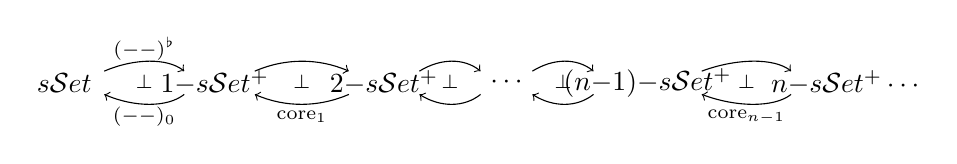
\begin{tikzpicture}[x=1.7em,y=1.4em]
  \node (s) at (0,0)    {$\sSet$};
  \node (a) at (3.2,0)  {$1\text{-}\sSet^{+}$};
  \node (b) at (6.8,0)  {$2\text{-}\sSet^{+}$};
  \node (d) at (9.4,0)  {$\cdots$};
  \node (c) at (12.4,0) {$(n{-}1)\text{-}\sSet^{+}$};
  \node (e) at (16.6,0) {$n\text{-}\sSet^{+}\cdots$};
  \draw[->] (0.85,0.3) .. controls (1.5,0.64) and (2.2,0.64) .. (2.55,0.3);
  \node at (1.7,0.88) {$\scriptstyle(\text{--})^{\flat}$};
  \node at (1.7,0.02) {$\scriptstyle\bot$};
  \draw[->] (2.55,-0.3) .. controls (2.2,-0.64) and (1.5,-0.64) .. (0.85,-0.3);
  \node at (1.7,-0.88) {$\scriptstyle(\text{--})_{0}$};
  \draw[->] (4.05,0.3) .. controls (4.7,0.64) and (5.4,0.64) .. (6.05,0.3);
  \node at (5.05,0.02) {$\scriptstyle\bot$};
  \draw[->] (6.05,-0.3) .. controls (5.4,-0.64) and (4.7,-0.64) .. (4.05,-0.3);
  \node at (5.05,-0.88) {$\scriptstyle\mathrm{core}_{1}$};
  \draw[->] (7.55,0.3) .. controls (8.0,0.64) and (8.5,0.64) .. (8.85,0.3);
  \node at (8.2,0.02) {$\scriptstyle\bot$};
  \draw[->] (8.85,-0.3) .. controls (8.5,-0.64) and (8.0,-0.64) .. (7.55,-0.3);
  \draw[->] (9.95,0.3) .. controls (10.4,0.64) and (10.9,0.64) .. (11.25,0.3);
  \node at (10.6,0.02) {$\scriptstyle\bot$};
  \draw[->] (11.25,-0.3) .. controls (10.9,-0.64) and (10.4,-0.64) .. (9.95,-0.3);
  \draw[->] (13.55,0.3) .. controls (14.3,0.64) and (15.1,0.64) .. (15.45,0.3);
  \node at (14.5,0.02) {$\scriptstyle\bot$};
  \draw[->] (15.45,-0.3) .. controls (15.1,-0.64) and (14.3,-0.64) .. (13.55,-0.3);
  \node at (14.5,-0.88) {$\scriptstyle\mathrm{core}_{n-1}$};
\end{tikzpicture}
\end{center}

在极限情形，我们还考虑伴随
\begin{center}
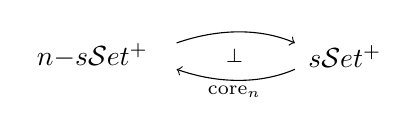
\begin{tikzpicture}[x=1.9em,y=1.4em]
  \node (n) at (0,0) {$n\text{-}\sSet^{+}$};
  \node (s) at (4.8,0) {$\sSet^{+}$};
  \draw[->] (1.6,0.34) .. controls (2.4,0.72) and (3.2,0.72) .. (3.85,0.34);
  \node at (2.7,0.02) {$\scriptstyle\bot$};
  \draw[->] (3.85,-0.34) .. controls (3.2,-0.72) and (2.4,-0.72) .. (1.6,-0.34);
  \node at (2.7,-0.92) {$\scriptstyle\mathrm{core}_{n}$};
\end{tikzpicture}
\end{center}
其中 $\mathrm{core}_{n}X\hookrightarrow X$ 是只包含那些「其维数大于 $n$ 的
诸面皆被标记」的单纯形的单纯子集。由伴随，这些\trFunctor{}把
$(n{+}1)$-复状单纯集载为 $n$-复状单纯集（见\cref{ex:n-core-complicial}）。
由于诸\trLeftAdjoint{}保持诸\trMonomorphism{}与诸\trProduct，这足以验证这些
伴随是 Quillen 的。\cref{cor:cartesian-closed-cosmos}现在诱导出所需的诸%
\trInfinityCosmos，而\cref{cor:right-quillen-adjunction-biequivalence}提供了
诸\trCosmological{}核函子。
\end{proof}

基于 Hirschowitz–Simpson \cite{bib56} 与 Pellissier \cite{bib90} 的既往工作，
Simpson 把\trSegalCategories{}之\trModelStructure{}的构造加以迭代
\cite[\S19.2-4]{bib116}。当基模型范畴取为 Quillen 的\trKanComplex{}之%
\trModelStructure{}时，第 $n$ 次迭代定义了诸 \textbf{Segal $n$-\trCategory}
（Segal $n$-categories），尽管 Simpson 也考虑了更一般的模型范畴论基。在适当
的假设之下——Segal $n$-范畴的情形正满足它们——如此产生的\trModelStructure{}%
是\trCartesianClosed{}且一切对象皆\trCofibrant，这强烈暗示：存在一座由其%
\trFibrant{}对象所张成的\trInfinityCosmos，即诸 Reedy 纤维性的 Segal
$n$-\trCategory。我们把对这一点的确证留给有兴趣的读者作为练习。

\subsection*{练习}

\begin{exercise}\label{ex:rezk-isofibration-formulation}
给出\cref{def:rezk-objects}中用于定义\trRezkIsofibration{}概念的诸条件 (i)、(ii)
与 (iii) 的「相对类比」的一个显式表述。
\end{exercise}

\begin{exercise}\label{ex:segal-n-category-cosmos}
探究 Hirschowitz 与 Simpson 的诸 Segal $n$-\trCategory{} \cite{bib56} 之上的
潜在\trInfinityCosmos{}结构。
\end{exercise}

\begin{exercise}\label{ex:cosmological-biequivalence-search}
搜寻本节所构造的诸\trInfinityCosmos{}之间的诸\trCosmologicalBiequivalence
（并请把你的发现与作者分享）。
\end{exercise}

